
\documentclass[border=10pt]{standalone}

% ----------------------------
\usepackage{tikz}
\usepackage{fancyhdr}

% ----------------------------
\usetikzlibrary{arrows,shapes,positioning,calc}
\tikzset{
  % Define standard arrow tip
  >=stealth',
  % Define style for boxes
  box/.style={
    rectangle,
    rounded corners,
    draw=black, very thick,
    text width=7.5em,
    minimum height=2em,
    text centered},
  % Define round style
  round/.style={
    ellipse, draw, thick,
    node distance=1cm,
    minimum height=5mm
  },
  % Define arrow style
  arrow/.style={
    ->,
    thick,
    shorten <=2pt,
    shorten >=2pt,},
  % line
  line/.style = {draw, -stealth', thick},
}

% Circle with arrow
\def\circledarrow#1#2#3{ % #1 Style, #2 Center, #3 Radius
\draw[#1,->] (#2) +(80:#3) arc(80:-260:#3);
}

% ----------------------------
\begin{document}

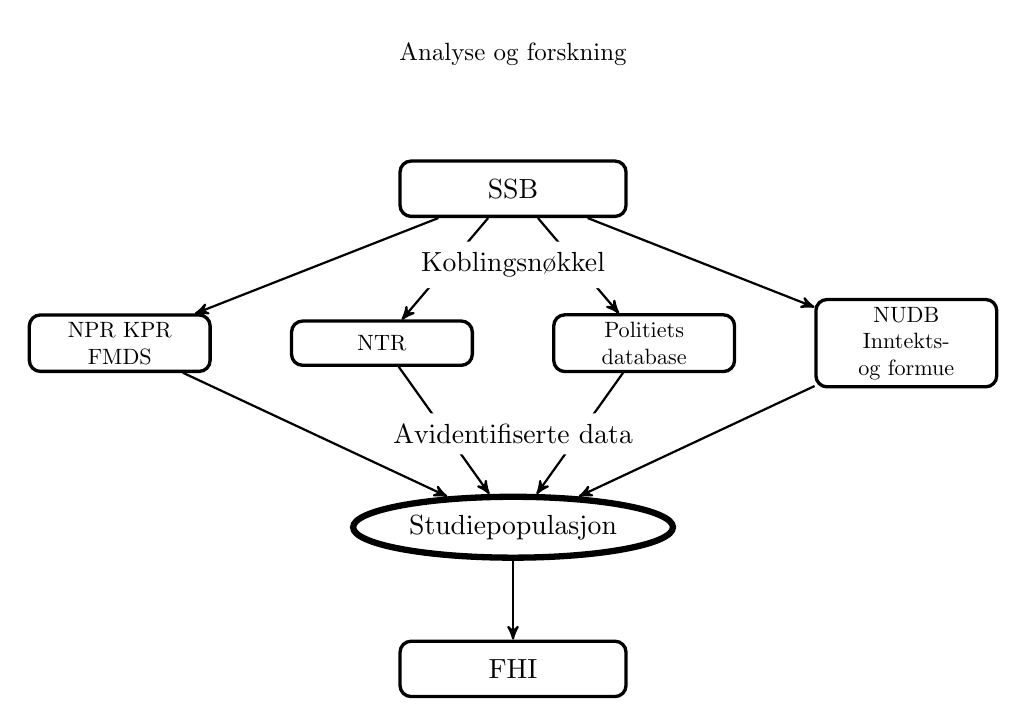
\begin{tikzpicture}[node distance=1cm, auto]
  % nodes
  % \node[box, text width=3em] (ssb) {SSB};
  \node[box, scale=.8, align=center] (hdir) {NPR KPR \\ FMDS};
  \node[box, right=of hdir, scale=.8] (ntr) {NTR};
  \node[box, right=of ntr, scale=.8] (politi) {Politiets database};
  \node[box, right=of politi, scale=.8, align=center] (nudb) {NUDB \\ Inntekts- og formue};
  \node[above=1.5 of ntr] (dum1) {};
  \node[above=1.5 of politi] (dum2) {};
  \node[box] at ($(dum1)!0.5!(dum2)$) (ssb) {SSB};
  \path[line] (ssb) -- (hdir);
  \path[line] (ssb) -- (ntr);
  \path[line] (ssb) -- (politi);
  \path[line] (ssb) -- (nudb);
  \node[box, draw=white, below=.3 of ssb, text width=7em, fill=white, minimum height=1]
  (txt) {Koblingsnøkkel};
  \node[box, draw=white, above=of ssb, text width=10em, scale=.9] (title) {Analyse og forskning};
  \node[round, line width=0.8mm, below=3.5 of ssb] (pop) {Studiepopulasjon};
  \path[line] (hdir) -- (pop);
  \path[line] (ntr) -- (pop);
  \path[line] (politi) -- (pop);
  \path[line] (nudb) -- (pop);
  \node[box, draw=white, above=.5 of pop, text width=10em, fill=white, minimum height=1]
  (txt) {Avidentifiserte data};
  \node[box, below=of pop] (fhi) {FHI};
  \path[line] (pop) -- (fhi);
\end{tikzpicture}

\end{document}
